\section{Estado del arte y antecedentes}

\subsection{Estado del arte del problema a tratar} \label{sec_estado_arte_problema}

El problema de la estimación de la edad a partir de restos óseos ya se ha tratado en distintas ocasiones, desde modificaciones a la propuesta de Todd, propuestas de como automatizar la estimación utilizando las características que proponía Todd, hasta estudios que utilizaban técnicas de visión por computador para recoger y procesar las características de los restos.

En 1990, J. M. Suchey y S. Brooks propusieron una modificación a la propuesta de Todd \cite{sucheyBrooks}, en la que evaluaban $1225$ restos óseos y llegaban a la conclusión de que era posible reducir las diez fases propuestas por Todd a seis fases, modificando el criterio de cada una de las fases y añadiendo cierto error marginal, aunque con un $95\%$ de confianza con los nuevos intervalos propuestos. Esta modificación es una de las más aceptadas por la comunidad científica, aunque la mayor parte de trabajos siguen utilizando las fases propuestas por Todd.

Uno de los más relevantes es un estudio publicado en el año 2015 en la revista \textit{Journal of forensic sciences} \cite{modelandoHuesos3D}, en el que se escaneaban los restos tomados como muestras para la variación de la sínfisis púbica y con esta variación realizar la estimación de la edad utilizando un modelo de regresión lineal y las seis fases propuestas por Suchey y Brooks. El conjunto de datos utilizado en este experimento se compone de $41$ esqueletos de personas estadounidenses y logran obtener una raíz del error cuadrático medio de unos $17.15$ años.

\begin{figure}[H]
	\centering
	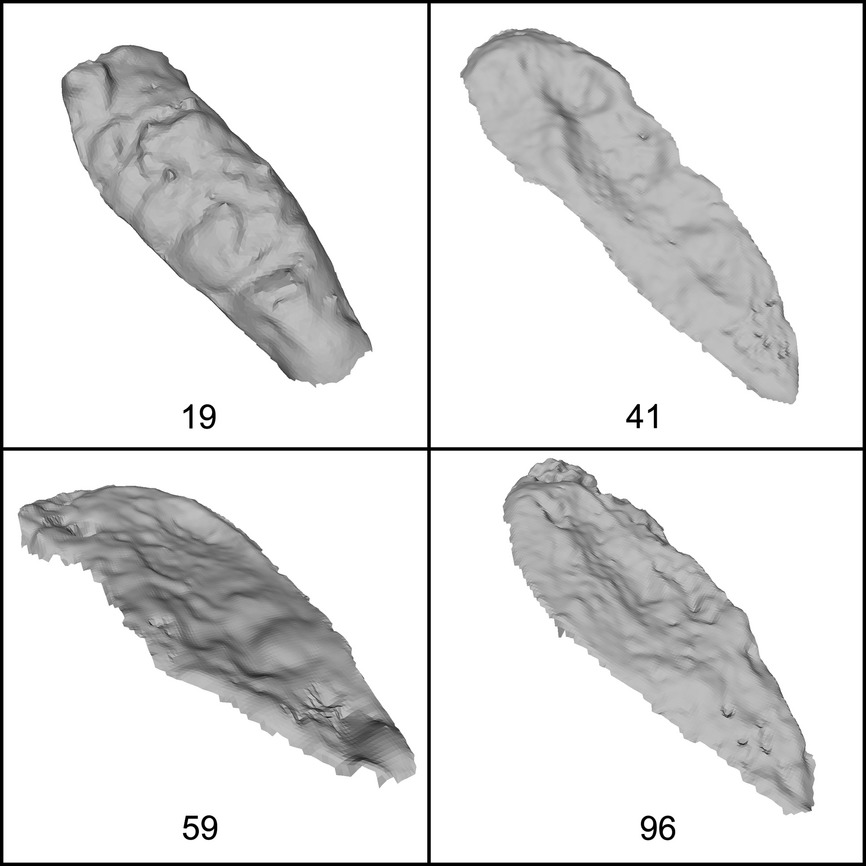
\includegraphics[scale = 0.4]{escaneo_huesos.jpg}
	\caption{Visualización del escaneo de la sínfisis púbica en cuatro individuos. La edad de la muerte aparece en la parte inferior de cada imagen. Imagen obtenida de \cite{modelandoHuesos3D}.}
	\label{fig:escaneo_huesos}
\end{figure}

Ese mismo año, los mismos autores presentaron una mejora \cite{mejoraModelandoHuesos3D} en la que, en lugar de utilizar la variación total de la sínfisis púbica, utilizaban la flexión de un plano de forma que dicho plano coincida con la superficie del hueso. De esta forma, utilizando un conjunto de datos similar a su experimento anterior y la curvatura de la sínfisis púbica entrenaron un modelo de regresión lineal con el que obtuvieron una raíz del error cuadrático medio de unos $19$ años.

A finales de 2015, Beatrix Dudzik y Natalie R. Langley, de la Universidad de Tennessee y la Universidad Lincoln Memorial, propusieron \cite{componentBased} varios modelos basados en árboles de decisión y regresión logística multinomial. Para estos experimentos utilizaron 5 características de la sínfisis púbica de 47 individuos de entre 18 y 40 años. Obtuvieron muy buenos resultados, con una tasa de acierto del $94\%$ aunque solo utilizaban 3 de las 6 fases propuestas por Suchey y Brooks.

\begin{figure}[H]
	\centering
	\begin{subfigure}{.5\textwidth}
	  \centering
	  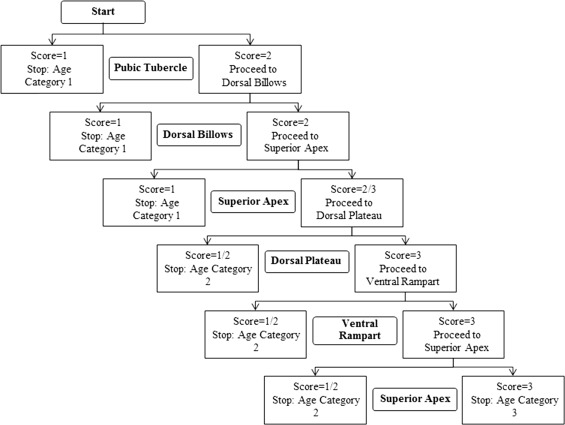
\includegraphics[scale = 0.7]{cita_7_arbol.jpg}
	  \caption{Árbol de decisión implementado en \cite{componentBased}}
	  \label{fig:arbol_c7}
	\end{subfigure}%
	\begin{subfigure}{.5\textwidth}
	  \centering
	  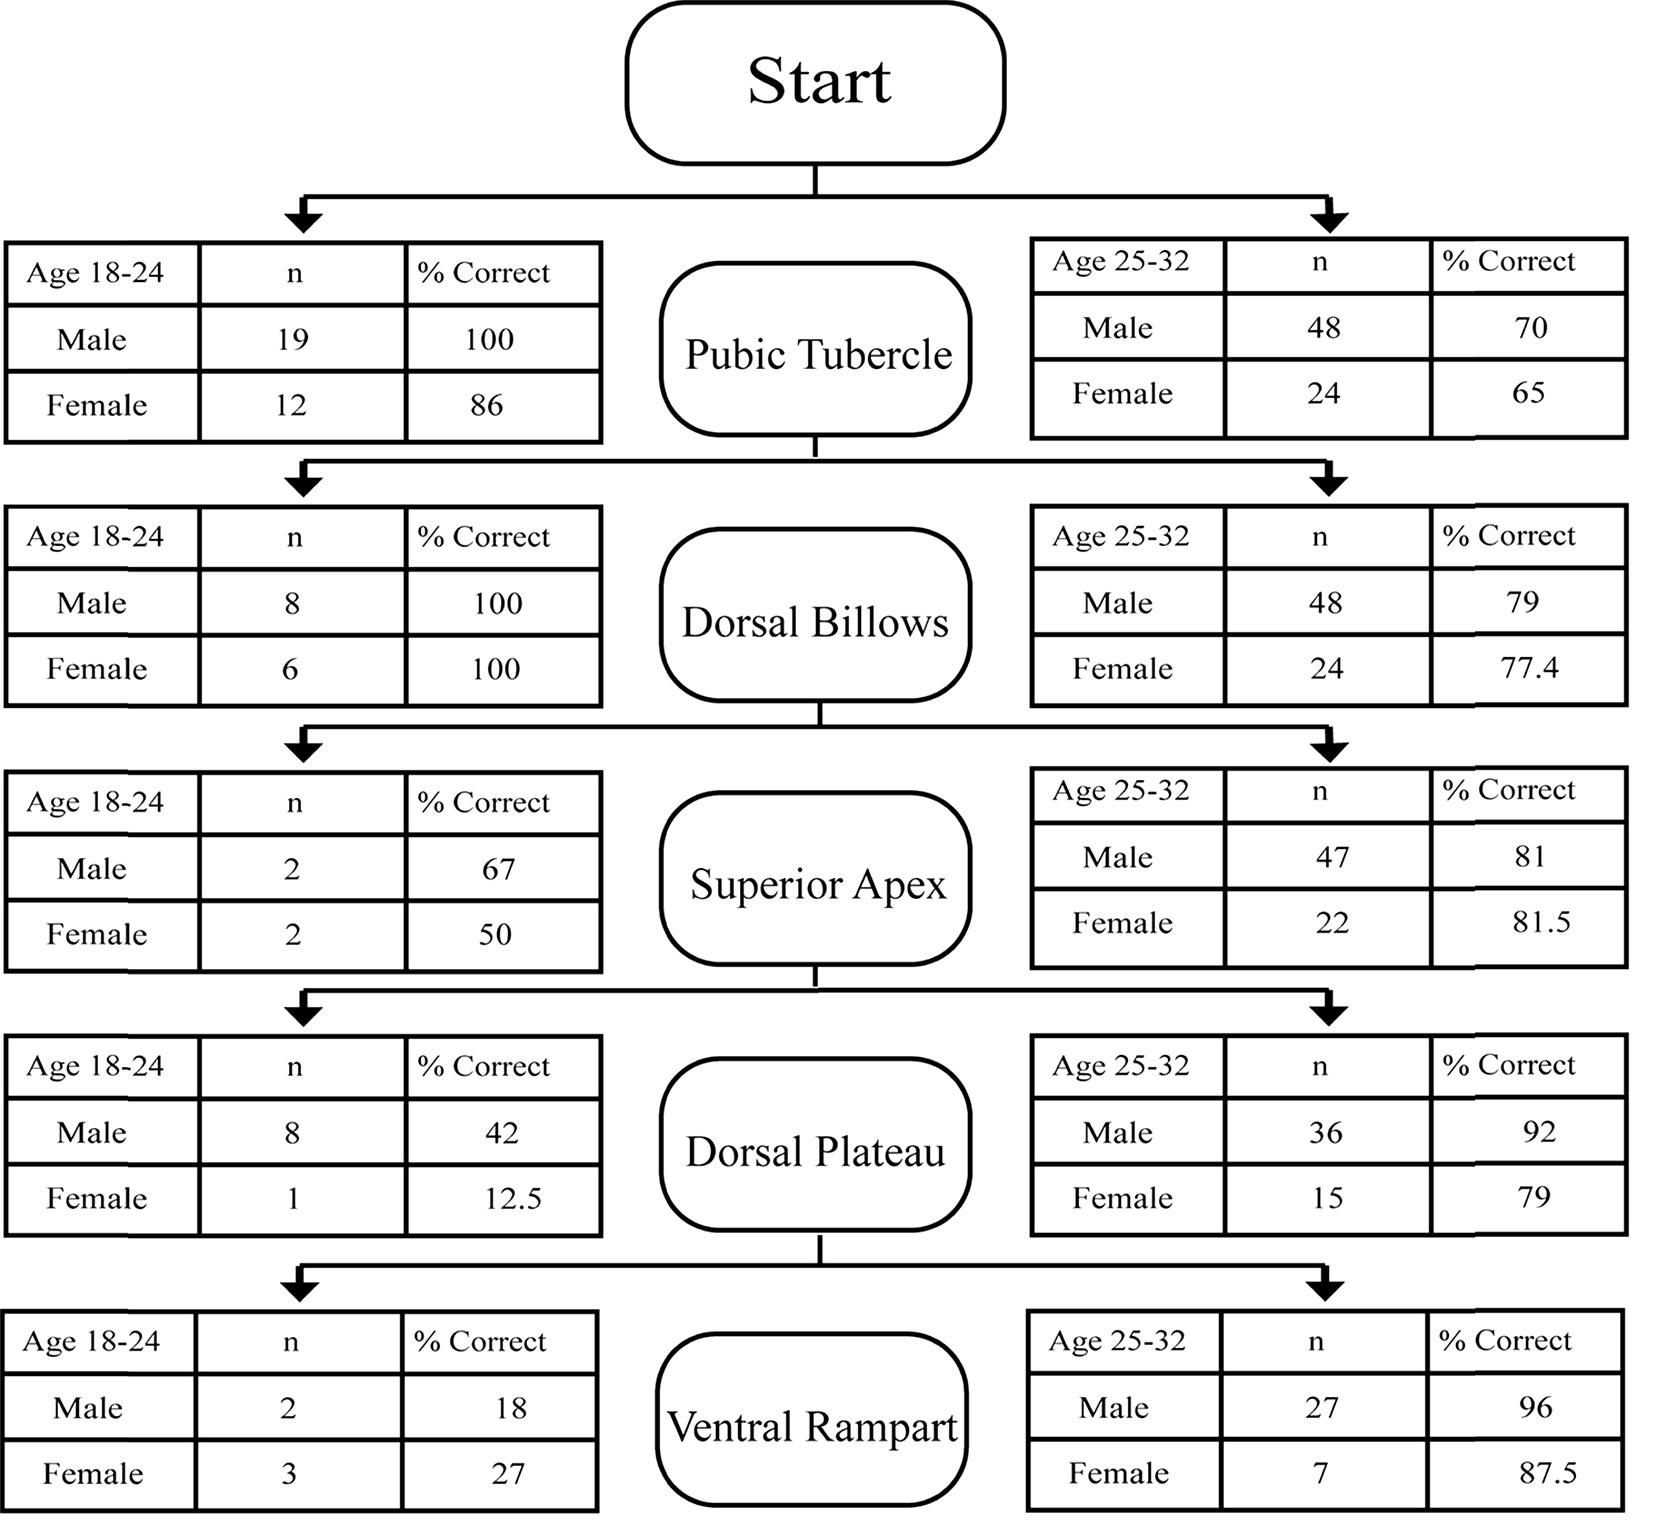
\includegraphics[scale = 0.8]{cita_7_ejemplo_dos_fases.jpg}
	  \caption{Porcentaje de acierto para la fase 1 y 2 de \cite{componentBased}.}
	  \label{fig:acierto_cita7}
	\end{subfigure}
	\caption{Imágenes obtenidas de \cite{componentBased}.}
	\label{fig:arboles_cita7}
\end{figure}



Más adelante, en 2018, varios investigadores de la República Checa publicaron un trabajo \cite{estimacionHuesosCadera} en el que, con un conjunto de $941$ restos óseos de personas de distinta raza entre 19 y 100 años, utilizando datos de los huesos de la cadera estudiaban las características comunes y las que diferenciaban las distintas edades, y consideraban 9 modelos distintos para realizar una estimación, desde un sistema de puntuación tradicional, utilizando la variación entre los huesos, distintos de regresión lineal, árboles de decisiones o redes neuronales artificiales. De estos modelos se llega a la conclusión que el mejor es un modelo de regresión multinomial, con el que obtienen una raíz del error cuadrático medio de unos $12.5$ años.

En 2017 investigadores de la Universidad de Granada publicaron un artículo preliminar de cara a obtener un modelo descriptivo basado en reglas con el que realizar la estimación de la edad a partir de la sínfisis púbica \cite{fuzzyAgeEstimation}. Utilizando $74$ muestras clasificadas manualmente consiguen entre 17 y 20 reglas utilizando árboles de decisión difusos que consiguen un error absoluto medio de $1.68$ años, aunque el resultado no es totalmente fiable debido a que no consiguen reglas para algunas fases propuestas por Todd.

Más adelante, en 2021, este mismo equipo con la ayuda de investigadores de la Universidad de Cordoba publicaron una continuación de su estudio \cite{NSLVOrdAge}. En este caso, utilizando el mismo conjunto de datos que utilizaremos nosotros, aplicando técnicas de balanceo y sobremuestreo de datos para resolver problemas relativos a dicho conjunto de datos, han enfocado el problema como un problema de clasificación ordinal. Utilizando el software NSLVOrd \cite{NSLVOrd}, un algoritmo de clasificación ordinal basado en el enfoque de aprendizaje de reglas de forma iterativa publicado por investigadores de la Universidad de Granada en 2016, son capaces de obtener una raíz del error cuadrático medio de $12.34$ años utilizando 34 reglas para las distintas fases. Este es, hasta este momento, el mejor resultado del estado del arte de este problema, y además en este estudio se discute sobre la importancia de las características a observar en la sínfisis púbica propuestas por Todd, llegando a la conclusión de que ciertas características nunca se utilizan, y por lo tanto no entran en juego a la hora de realizar la estimación de la edad.


% Comentar el enfoque de Gilbert y McKern y diferenciar ambos enfoques

Otro enfoque de este problema es el propuesto por McKern y Stewart en el año 1957 \cite{primeraPropuestaMcKern} y que luego ampliarían en 1973 junto a Gilbert \cite{propuestaGilbert}. En lugar de resolver el problema con un enfoque de clasificación, proponían un método en el que se le asignan valores numéricos a cada uno de los distintos posibles estados de cada característica observada en la sínfisis púbica, y con esos valores conseguir una fórmula que estimase la edad. En este trabajo utilizaremos este enfoque de cara a tratar este problema como un problema de regresión. En la siguiente sección haremos una presentación más detallada de este método.

Uno de los primeros trabajos que aplico este enfoque fue un estudio de la Universidad de Tokio \cite{primerTrabajoGilbert}. Los autores utilizan una extensión de la regresión lineal, regresión lineal múltiple, ya que utilizan siete características de la sínfisis púbica y una constante de cara a obtener fórmula que les sea capaz de estimar la edad. Tras los distintos experimentos, consiguen obtener unos resultados bastante buenos aunque, como los propios autores indican, el rango de edades con el que se ha trabajado es bastante limitado, siendo solo entre 18 y 38 años y solo contando con 135 muestras de sínfisis púbica.

Años más tarde, en 1995, Investigadores del departamento de Medicina Forense del All India Institute of Medical Sciences en Nueva Delhi, India, utilizarán este trabajo para aplicarlo a 41 individuos de entre doce y setenta y cinco años, comparando los resultados utilizando regresión lineal múltiple con el sistema de clasificación de Todd \cite{estudioComparandoGilbertTodd}. En este trabajo se logran obtener resultados significativamente mejores que con la propuesta de Todd, además de sumarse a las conclusiones de otros trabajos, que aunque tomen un enfoque distinto, se podrían modificar las fases propuestas por Todd, ya que se observan como algunas de las variables tienden a zonas entre dos fases de Todd, además de encontrar algunas de las características de la sínfisis púbica irrelevantes a la hora de estimar la edad en muchas de las fases.


\subsection{Enfoque de Gilbert y McKern}

En el enfoque propuesto por McKern en 1957 \cite{primeraPropuestaMcKern} y más tarde ampliado por el mismo autor y Gilbert en 1973 \cite{propuestaGilbert} se propone analizar tres componentes:

\begin{enumerate}
	\item Superficie dorsal de la sínfisis púbica.
	\item Rampa ventral.
	\item Anillo de la sínfisis.
\end{enumerate}

A cada una de estas componentes le corresponde un valor entre cero y cinco, dependiendo de su estado de desarrollo, de forma que se obtengan como resultado tres valores. De la suma de estos tres valores se obtendrá un resultado, que dependiendo del valor obtenido se le asignará un rango de edad que será la estimación.


\begin{figure}[H]
    \centering
	 \begin{subfigure}[b]{0.49\textwidth}
		 \centering
		 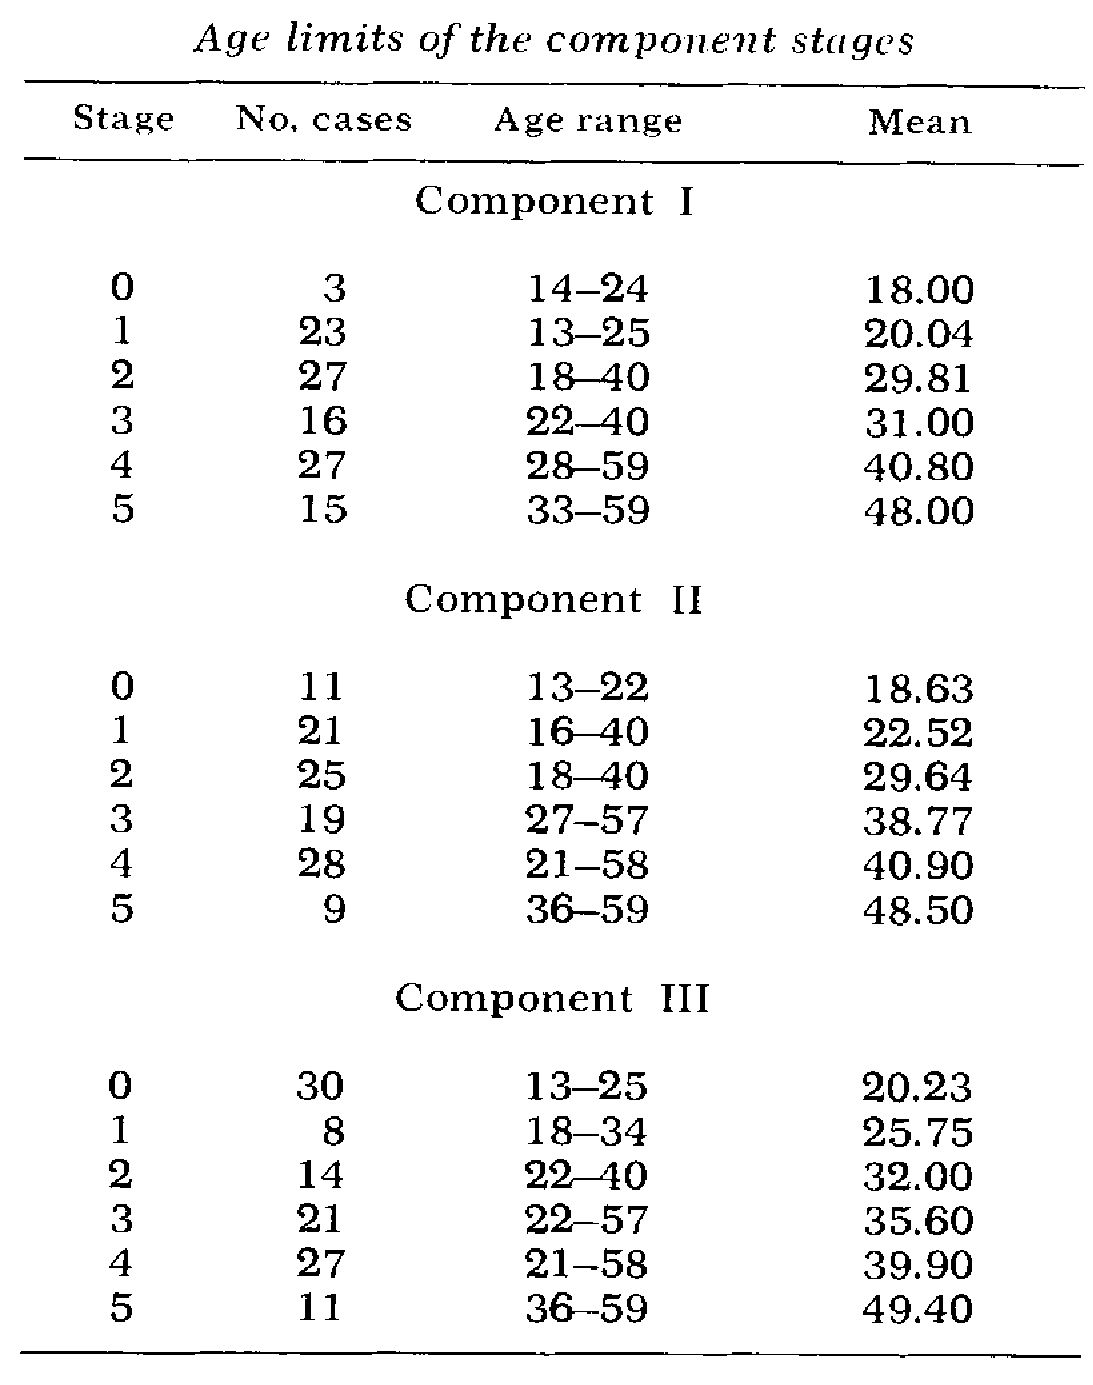
\includegraphics[width=0.8\textwidth]{componentes_gilbert.png}
		 \caption{Límite de edad para cada estado de las componentes.}
		 \label{fig:componentes_gilbert}
	 \end{subfigure}
	 \begin{subfigure}[b]{0.49\textwidth}
		 \centering
		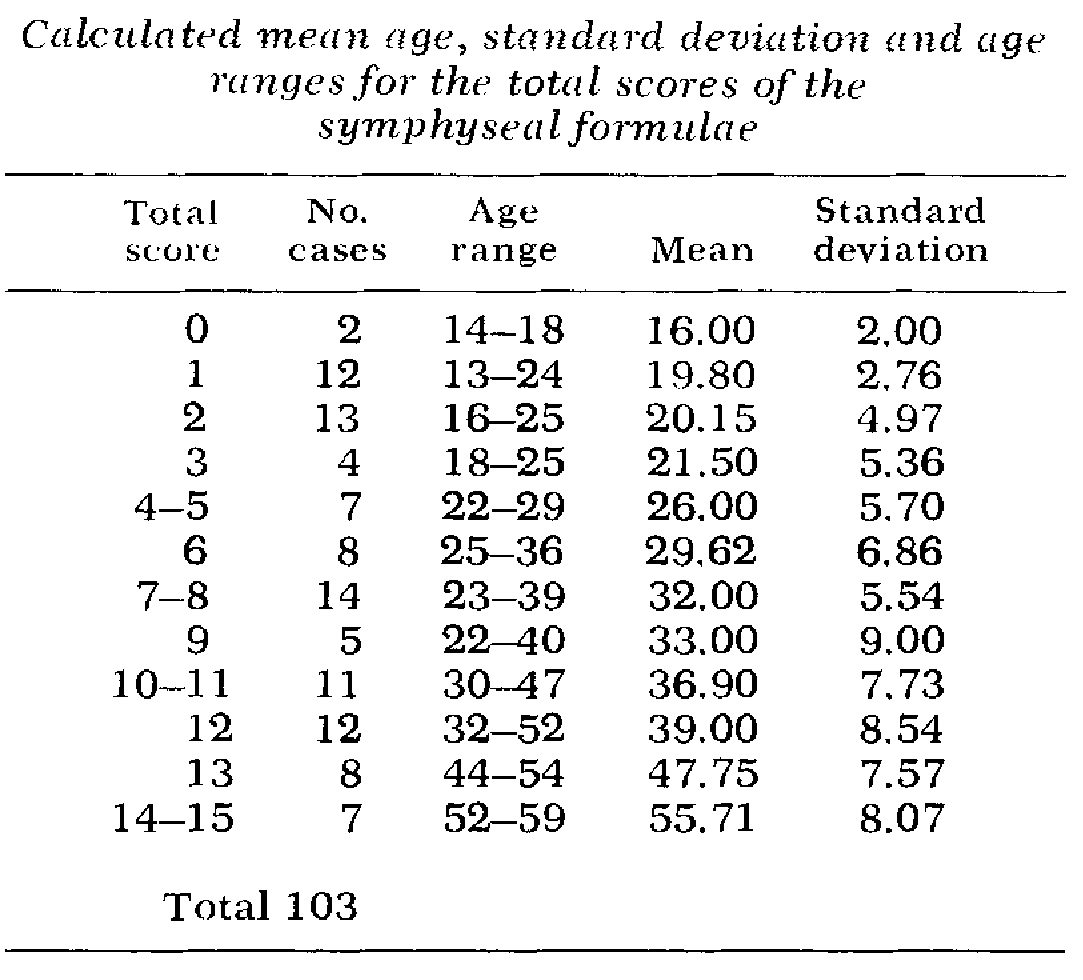
\includegraphics[width=0.8\textwidth]{mujeres_gilbert.png}
		\caption{Rangos de edades y puntuaciones asociadas en la propuesta de Gilbert y McKern.}
		\label{fig:mujeres_gilbert}
   \end{subfigure}
	\caption{Tablas obtenidas de \cite{propuestaGilbert}}
	\label{fig:gilbert}
\end{figure}

El trabajo de estos investigadores surge de la necesidad de revisar el método propuesto por Todd, así como de reducir el número de componentes observadas para realizar la estimación. También, en su segundo trabajo, se propone una adaptación del método para restos del pubis de mujeres, ya que debido a factores como el embarazo los estados de desarrollo propuestos en su primer trabajo hacen que sea más difícil obtener unos buenos resultados si los restos óseos pertenecen a una mujer.

Todo este trabajo fue recopilado por McKern en 1973 \cite{recopilacionMcKern}, donde se trata el problema, el enfoque propuesto, las diferencias a tener en cuenta si las muestras son de hombre o mujeres y se muestra una comparación con el método de Todd, mostrando como este enfoque, sin contradecir el trabajo de Todd, se trata de una mejor propuesta para obtener un modelo de estimación de la edad a través de los huesos del pubis.


\subsection{Regresión simbólica}

La regresión simbólica es un tipo de regresión que, a diferencia de otros tipos de regresiones como la lineal o la polinómica, es capaz de ajustar un modelo sin tener la información de como es la fórmula resultante, es decir, ajusta tanto los parámetros utilizados en la fórmula de la regresión como su forma. Esto permite que el modelo no se vea afectado por el sesgo del diseñador que construye dicho modelo para ajustarse a sus datos.

Uno de los trabajos donde claramente podemos ver las diferencias entre los distintos modelos de regresión es en \cite{analisisRegresionSimbolica}, donde hacen una comparación entre distintos tipos de regresión. De este trabajo podemos obtener que si se conoce el conjunto de datos y problema a tratar, así como la forma que puede tener la solución, se pueden conseguir mejores resultados si el modelo se ciñe a la fórmula que se estime oportuna a partir de ese conocimiento del problema, pero por otro lado, si se desconoce que forma tendrán las soluciones, así como el peso necesario de cada característica, la regresión simbólica aporta un gran valor a la hora de evitar un sesgo que con cualquier otra aproximación estaríamos obligados a añadir.

%  TODO : Ampliar esta seccion con mas papers y trabajos que hablen sobre regresión simbólica

\subsection{Programación Genética}

La Programación Genética apareció como una adaptación de los algoritmos evolutivos para representar programas de ordenador como cromosomas en una estructura de árbol. A pesar de que su aparición fue en 1985 no fue hasta principios de 1990 cuando este método comenzó a ser más utilizado gracias a John Koza \cite{kozaGP}.

La forma en la que la Programación Genética expresa los cromosomas permite resolver problemas de distintos tipos dando soluciones sencillas de interpretar, por este motivo este algoritmo y sus variaciones han sido bastante utilizadas.

Uno de los primeros trabajos fue de publicado por P. A. Whigham en 1995 \cite{PGgramaticas}, en el que se utiliza una gramática inicial libre del contexto para generar expresiones a utilizar en el algoritmo, y que durante el entrenamiento el algoritmo complete la gramática y la amplíe con nuevas reglas, siendo un claro ejemplo de aprendizaje incremental.

La Programación Genética nos ofrece un algoritmo muy bueno para problemas en los que los resultados son variables, no se conoce a priori la forma que tendrá el resultado, además de todas las ventajas de los algoritmos evolutivos. Por este motivo, una de las aplicaciones principales de este algoritmo es la regresión simbólica, ya que Programación Genética permite que las expresiones no tengan una forma fija, si no que se aprenda la forma de estas expresiones.

La principal forma de conseguir que Programación Genética trabaje con regresión simbólica es modificar los cromosomas propuestos por John Koza, en lugar de ser programas de ordenador, generador por gramáticas, los cromosomas serán expresiones matemáticas, manteniendo siempre la forma de árbol. Esta modificación es tan simple por reemplazar la gramática por una gramática que genere expresiones matemáticas, con los operadores que se estimen oportunos.



En 1995, investigadores de la Universidad de Georgia publicaban un artículo \cite{primerGAP} en el que proponían utilizar Programación Genética para hacer regresión simbólica, es decir, aprender una fórmula matemática estructurada como un árbol. En este trabajo se mencionan los principales problemas de la Programación Genética para regresión simbólica, todos ellos derivados de que este algoritmo solo puede modificar la estructura de las expresiones, no su contenido como tal, no siendo capaz de trabajar con valores numéricos constantes, además de generar ramificaciones complejas para obtener cierta constante.

Un claro ejemplo de esto es que si en cierto nodo se necesita multiplicar un valor $a$ por la constante $2$, lo único que podrá modificar Programación Genética será la ramificación que se multiplica por $a$, y si no cuenta con una constante que sea el valor necesario, utilizará las constantes disponibles para hacer una expresión compleja cuyo resultado sea $2$.

Para resolver dichos problemas se propone una modificación del algoritmo, un algoritmo híbrido entre Programación Genética y un Algoritmo Genético, de ahí el nombre GA-P (Genetic Algorithm-Programming). Este algoritmo se basa en que cada individuo tendrá tanto el árbol de Programación Genética como un cromosoma habitual en un Algoritmo Genético, de forma que los nodos del árbol que representen una constante numérica tendrán asociados una posición en el cromosoma de la parte de Algoritmo Genético, de esta forma, se aprenderán tanto la estructura de la expresión con Programación Genética, como las constantes numéricas que intervienen en la expresión utilizando un Algoritmo Genético.

Más adelante esta variación de Programación Genética se utilizará en diversos trabajos, como el publicado por investigadores de la Universidad de Oviedo y la Universidad de Granada en 1999 \cite{GAPredElectrica}, donde utilizando este algoritmo consiguen unos resultados bastante buenos en dos problemas reales aplicando regresión simbólica.

Un año más tarde, en el año 2000, aunque ya existían trabajos en los que se utilizaba Programación Genética y algunas variantes de cara a realizar regresión simbólica, investigadores del Laboratorio Nacional de Computación Científica de Brasil publican un artículo \cite{PGregresionSimbolica} donde explican en detalle los distintos operadores necesarios.

En el año 2000, también investigadores de la Universidad de Granada, publicaron un trabajo donde utilizan GA-P para aprender consultas booleanas \cite{GAPFormulasBooleanas} en el que demuestran la versatilidad del algoritmo para distintos problemas, además de que las soluciones obtenidas son fácilmente interpretables.

%\subsection{Sistemas basados en reglas}


\newpage
